%
% einleitung.tex -- Beispiel-File für die Einleitung
%
% (c) 2020 Prof Dr Andreas Müller, Hochschule Rapperswil
%
% !TEX root = ../../buch.tex
% !TEX encoding = UTF-8
%
\section{Einleitung\label{ueberschall:Einleitung}}
\kopfrechts{Einleitung}
In diesem Paper werden die Strömungsgleichungen im Unter- und
Überschallgebiet diskutiert.
Im Unterschallgebiet wird die Strömungsgleichung unter gewissen
Vereinfachungen zu einer elliptischen partiellen Differentialgleichung
zweiter Ordnung
\begin{align*}
    \Delta u = \frac{\partial\,^2\,u}{\partial\,x\,^2} +
    \frac{\partial\,^2\,u}{\partial\,y\,^2} = 0, 
\end{align*}
auch bekannt als Laplace-Gleichung.
Hingegen im Überschallgebiet verändert sie sich zu einer hyperbolischen
partiellen Differentialgleichung zweiter Ordnung
\begin{align*}
    \frac{\partial\,^2\,u}{\partial\,x\,^2} -
    \frac{\partial\,^2\,u}{\partial\,y\,^2} = 0, 
\end{align*}
besser bekannt als die Wellengleichung.

Dies hat Jakob Ackeret in seiner Habilitationsschrift~\cite{Ackeret1928}
detailliert erklärt.
Jakob Ackeret, siehe Abbildung~\ref{fig:ackeret}, spielte eine bedeutende 
Rolle für die Forschung in der Schweiz und an der ETH Zürich, 
wo er als Leiter des Instituts für Aerodynamik arbeitete.
\begin{figure}
    \centering
    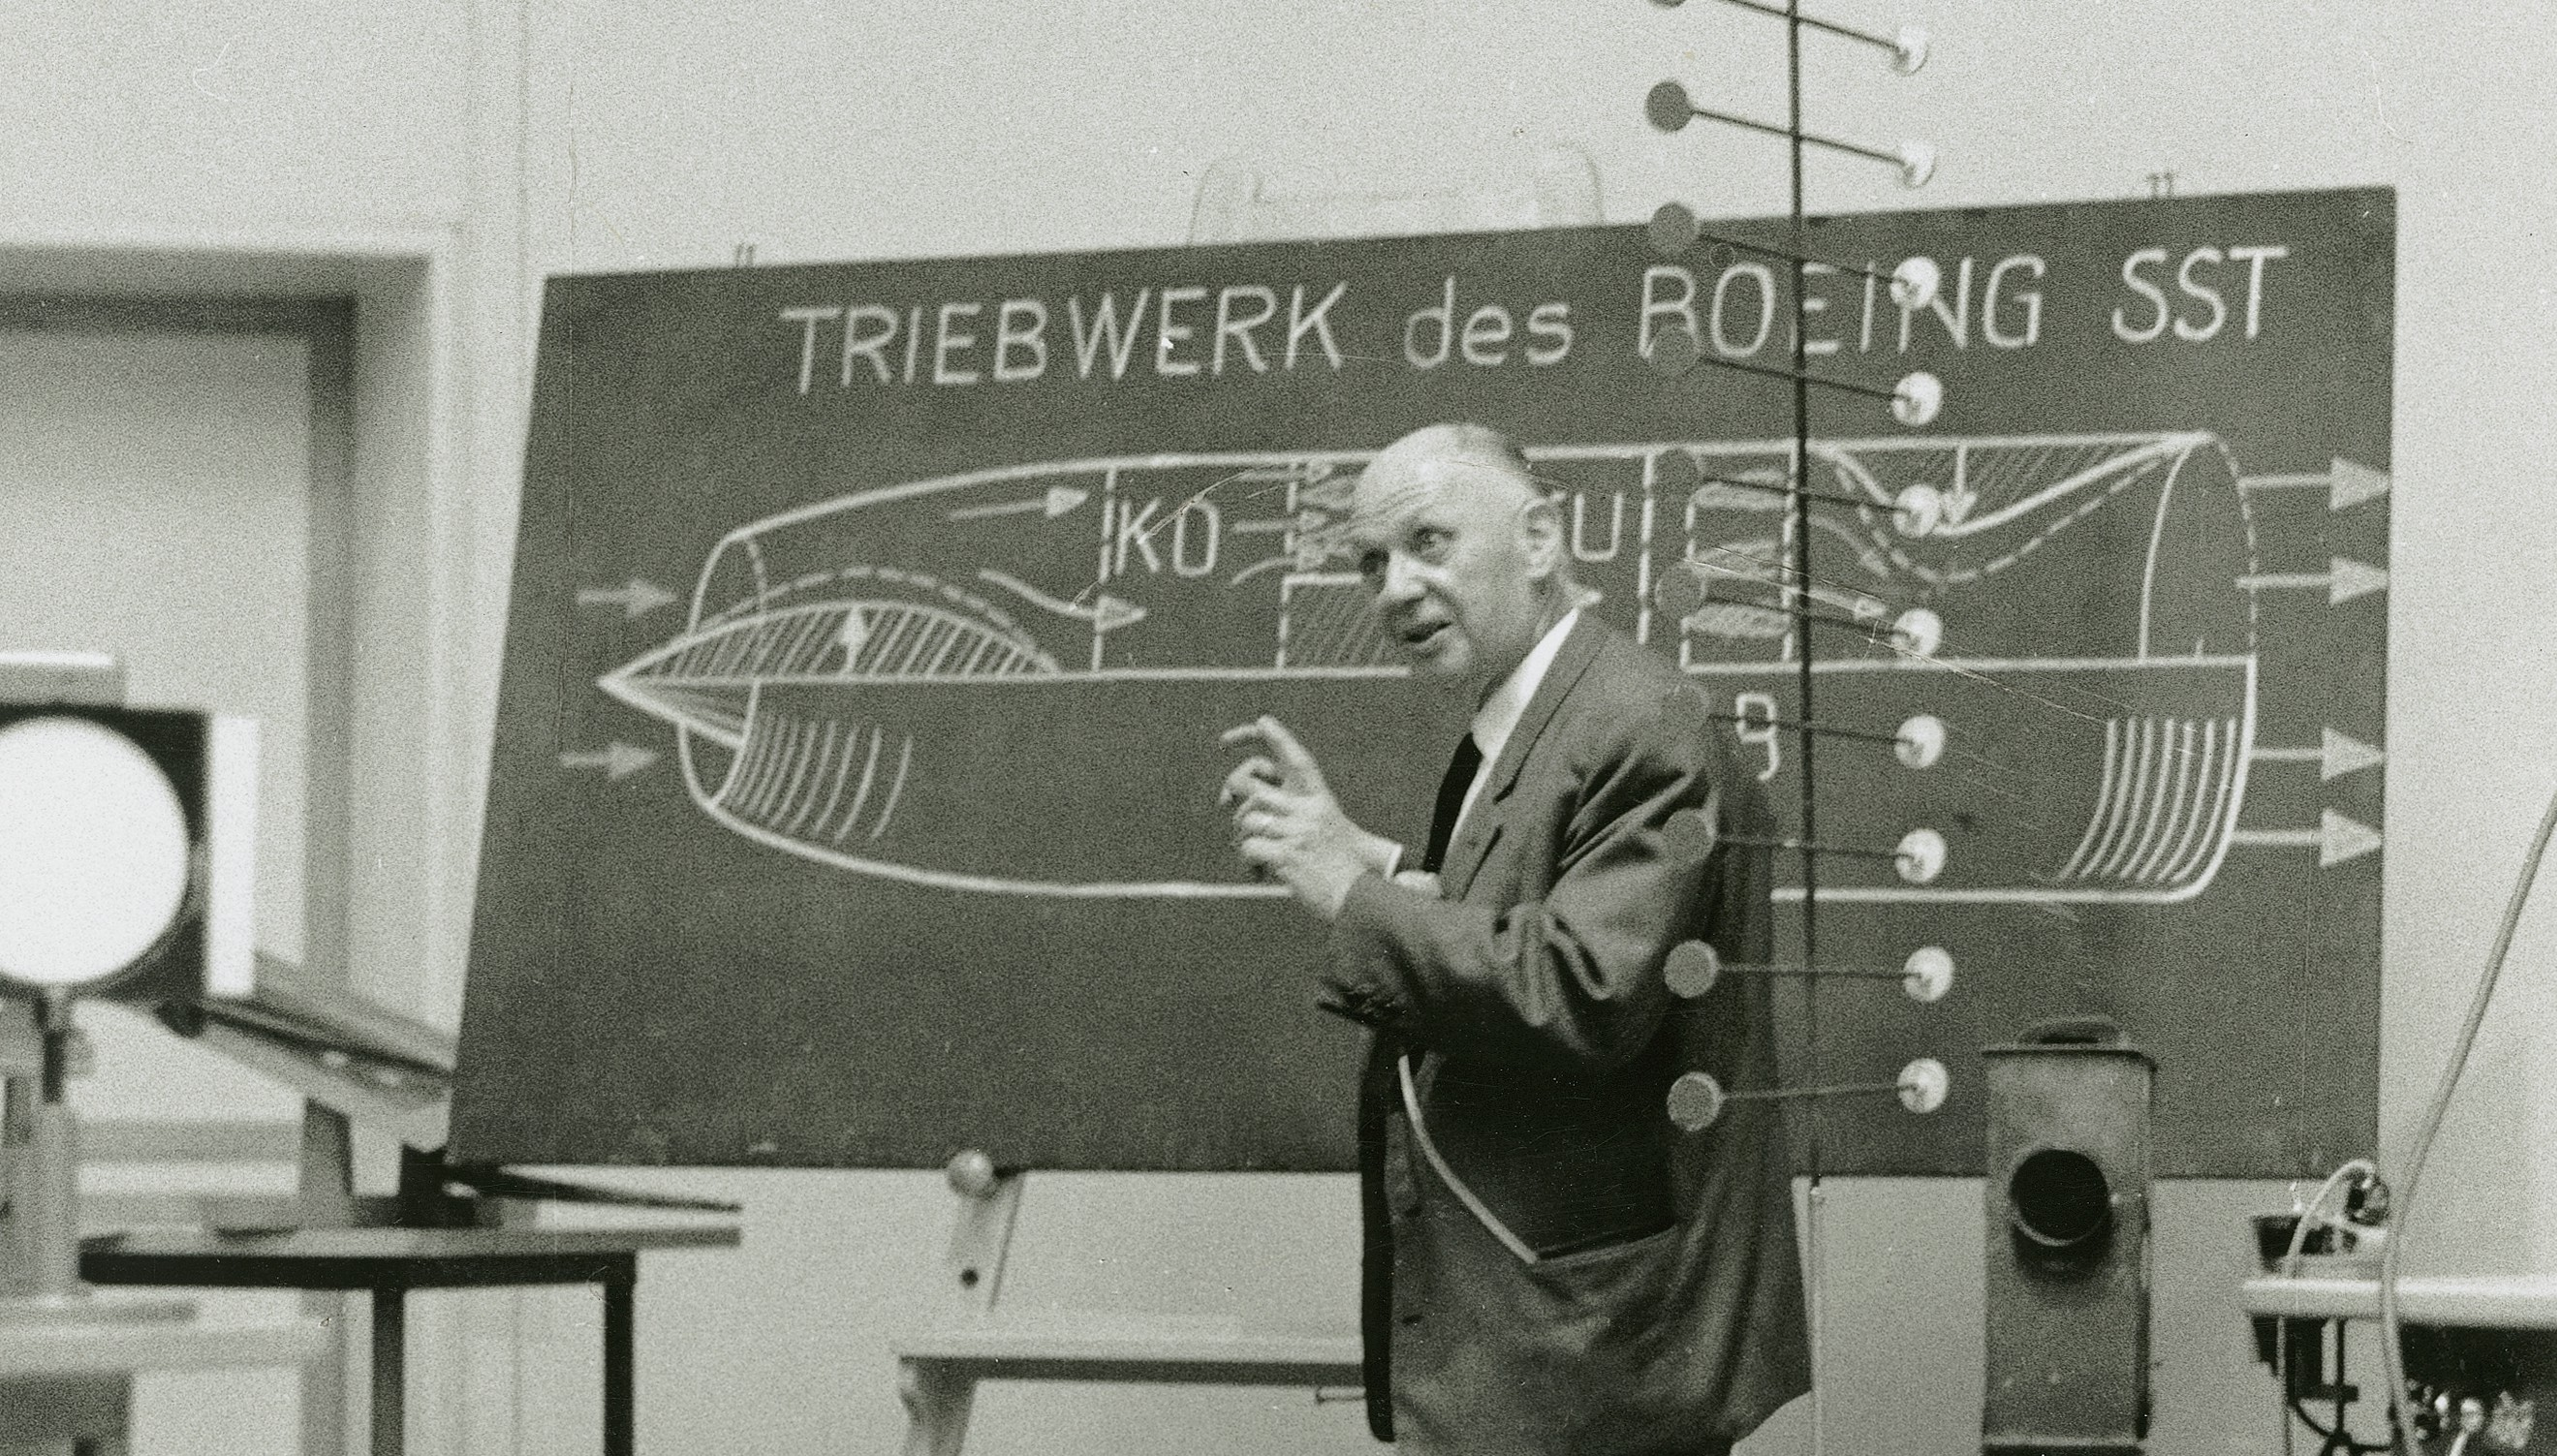
\includegraphics[width=\textwidth]{papers/ueberschall/figures/Jakob_Ackeret_1967.jpg}
    \caption{Professor Jakob Ackeret bei seiner Abschiedsvorlesung~\cite{AckeretFoto1967}.}
    ~\label{fig:ackeret}
\end{figure}
Dort errichtete er den weltweit ersten Überschallwindkanal 
mit geschlossenem Kreislauf, siehe Abbildung~\ref{fig:windkanal}.
Dies war ein entscheidender Meilenstein für 
die Entwicklung von Überschallflugzeugen.
\begin{figure}
    \centering
    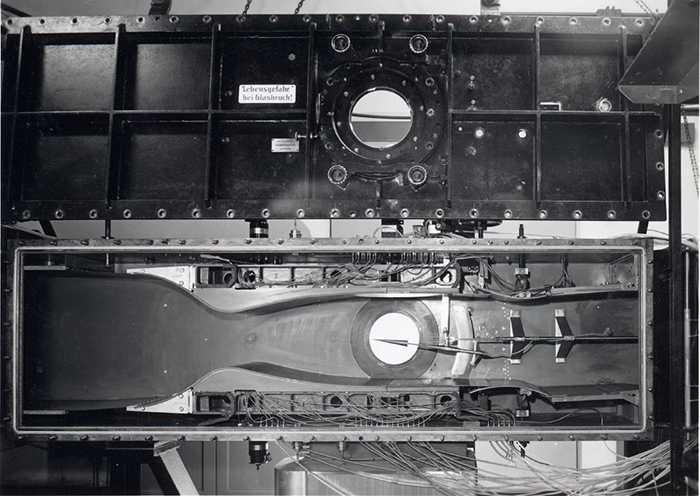
\includegraphics[width=\textwidth]{papers/ueberschall/figures/Windkanal.jpg}
    \caption{Der erste Überschallkanal mit geschlossenem Kreislauf~\cite{ETHeritage2020}.}
    ~\label{fig:windkanal}
\end{figure}

Die Gleichungen für die Überschallströmung fanden 
später unter anderem Anwendung bei der Suche nach Körperformen 
mit minimalem Luftwiderstand im Überschallbereich, 
wie der sogenannte Sears-Haack-Körper. 
Dieser Fragestellung wurde ein ganzes Buch gewidmet, 
insbesondere der Beitrag von Carlo Ferrari
\textit{Bodies of Revolution Having Minimum Pressure Drag}~\cite{Ferrari1965}.

